\section{Design}

\subsection{Hardware}

Systemet består af PSoC-Master som er forbundet til DevKit8000 med en 4-ledningers SPI-bus og forbundet til PSoC-XY, -Z og -Sensor med en 2-ledningers I2C-bus med eksterne pull-up modstande. Til test/debugning er der også brugt en UART forbindelse til at udlæse til Tera Term og en Nokia 5110 skærm til at aflæse indkommende og udgående kommuniaktion via SPI og I2C. På figur \ref{fig:psoc-master_topdesign} kan tilslutningerne for PSoC-Master ses.

% TopDesign PSoC-Master.
\begin{figure}[H] \centering
    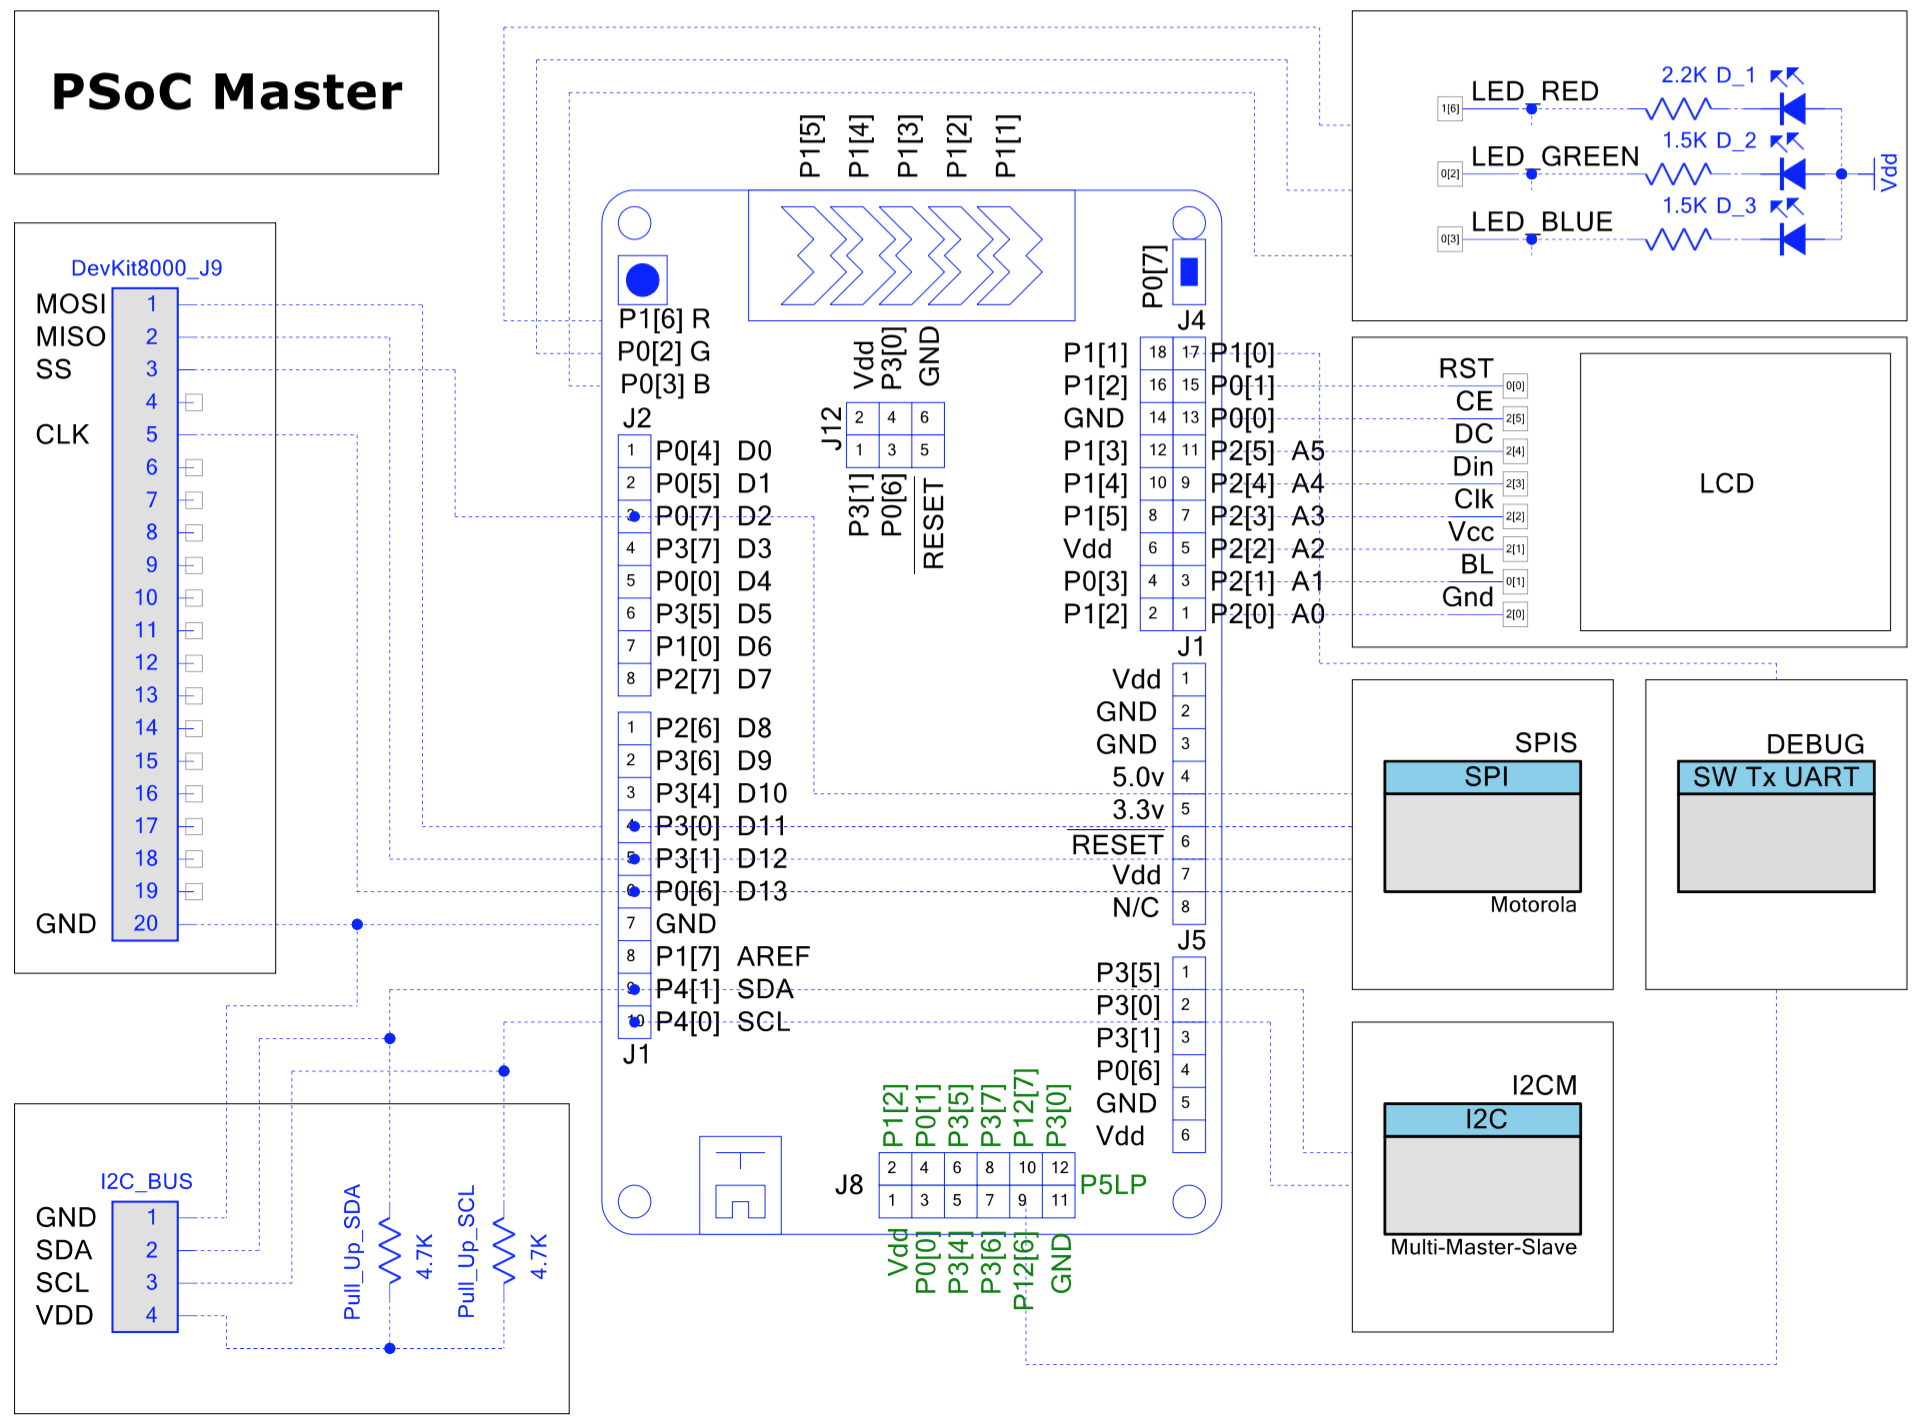
\includegraphics[width=\textwidth]{Filer/PSoC-Master_TopDesign.png}
    \caption{TopDesign PSoC-Master}
    \label{fig:psoc-master_topdesign}
\end{figure}

\subsubsection{Master-Blokken}
Systemet består af:
\begin{itemize}
	\item En PSoC\footcite{psoc}.
	\item Et Nokia 5110 display\footcite{nokia}.
\end{itemize}

Formålet med PSoC-Master er at den skal fungere som en "beskedcentral" mellem DevKit8000 og PSoC-XY, -Z og -Sensor.

Forbindelsen med DevKit8000\footcite{dk8000-addon} kører over SPI kommuniaktion, hvor DevKit8000 er SPI-master og PSoC-Master er SPI-slave.


\subsubsection{XY-Blokken}

Designet af XY blokken består af følgende 3 dele.

\begin{itemize}
    \item En PSoC\footcite{psoc}
    \item 4 stk. Stepper motor af typen (28BYJ-48) se databladet\footcite{28BYJ-48-5V} i bilag.
    \item 4 stk. Micro switches af typen (DM1-01P-30-3) se databladet\footcite{DM1-01P-30-3} i bilag.
\end{itemize}

For at kunne styre stepper motorerne er der implementeret en motorstyring. PSoC har 4 pins den sætter højt skiftevis, disse 4 pins giver et signal til motorstyringen, som alt efter hvilken pin der er aktiv, aktiveres en spole i motoren, som skifter polerne på en magnet. Dette sker ved at den tilslutter en stel forbindelse så der kan løbe en strøm i spolen. Magneten kan ved polskift få motoren til at bevæge sig. Ved at styre rækkefølgen af hvordan disse pins bliver sat høj kan man styre hvad vej motoren kører. Som ende stop på XY skinnerne er der blevet implementeret 4 switches/kontakter; 2 på X og 2 på Y. Kontakterne, ved aktivering, vil stoppe for den bevægelse der er i gang for at sikre systemets fortsatte drift. Yderligere bruges kontakterne ved kalibrering for at systemet kan registrere når lampen er nået til sine endepunkter på de pågældende skinner. 

Denne styring er stærkt inspireret af GFV\footcite{gfv}-øvelsen omkring stepmotorer.

\subsubsection{Z-Blokken}

Designet Z blokken består af følgende 3 dele.

\begin{itemize}
	\item En PSoC\footcite{psoc}.
	\item Én Stepper motor af typen (28BYJ-48) se databladet\footcite{28BYJ-48-5V} i bilag.
	\item Én Micro switch af typen (DM1-01P-30-3) se databladet\footcite{DM1-01P-30-3} i bilag.
\end{itemize}

Motoren til Z-aksen er styret på samme måde som motorerne for XY-delen.\footcite{documentation} Dvs. Motoren har 4 input pins + en 5 V VCC. Sættes de 4 input pins gentagende gange skiftevis til ground, i en bestemt rækkefølge, vil motoren kører rundt. Vælges den modsatte rækkefølge kører motoren baglæns.

Lampen hejses ned fra vognen med et fladt bånd. Køres lampen op vil den på et tidspunkt ramme en switch oppe under vognen. Til at signalere hvornår lampen er kørt langt nok ned, afhænger systemet af afstandssensoren, som sidder inde i lampen til at vurdere og markere hvornår en nedre grænse for Z-højden er nået.

\subsubsection{Sensor-Blokken}

Systemets sensorer er monteret direkte på bunden af vognen der kører på Y-aksen. Her er de forbundet til Z-vognprintet som giver den direkte forbindelse til PSoC-Sensor hvorfra de styres.

\subsection{Software}

\subsubsection{Kommunikation og databehandling}

Softwaren er fordelt ud på henholdsvis 1 Devkit8000 og 4 PSoC'er, med hver deres formål i produktet. Devkittet er brugerfladen, der viderebringer brugerinput og 1 af de 4 PSoC er beskedcentralen. Denne har til formål at distribuere input og output til de resterende PSoC'er baseret på de modtagene beskeder fra Devkittet. De resterende tre PSoC'er står for motorstyring i retning X, Y, Z samt styrer sensorerne.

Når et handlingsforløb påbegyndes, eventuelt ved tryk på devkittets touchskærm, vil inputtet blive tolket, sendt videre til beskedcentralen og derfra blive sendt videre til aktuelle PSoC-slave som har interesse i givne brugerinput. Givne PSoC-slave/r behandle dernæst disse data og produktets hardware vil skabe en respons. Denne procedure beskriver det generelle handlingsforløb fra Devkit8000 til hardware. 

Som eksempel på dette er der herunder opstillet en applikationsmodel, der beskriver kodeeksekveringen baseret på use-case 1 i dokumentationen. Denne use-case beskrive hvordan kalibrering af systemet bliver udført. For yderligere information om denne use-case, se dokumentationen sektion 2.3.1.


% {Applikationsmodel UC1
\begin{figure}[H] \centering
    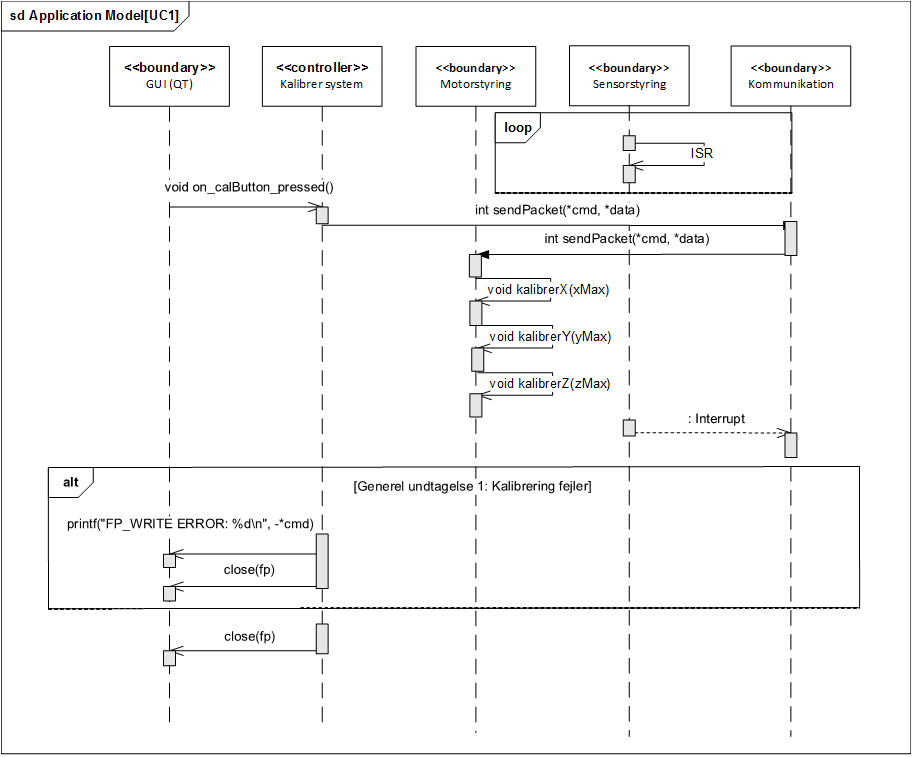
\includegraphics[width=\textwidth]{Filer/sdApplikationsmodelUC1.png}
    \caption{Applikationsmodel for UC1}
    \label{fig:sdUC1}
\end{figure}


\subsubsection{Devkit8000-Blokken}

Systemet består af:
\begin{itemize}
	\item Et Devkit8000\footcite{devkit}.
\end{itemize}

Devkit8000 har til formål at fungere som en fjernbetjening/styringsenhed til resten af systemet og være den del af systemet som brugeren aktivt skulle interagere med.

Devkit8000 indeholder en grafisk brugerflade (GUI) bestående af nogle grafiske elementer oprettet fra QT's designer. Disse elementer påvirkes live som et eventbaseret system, og er det brugeren kan se på Devkittets touchskærm. Når Devkittet påvirkes via touchskærmen bliver kode eksekveret i baggrunden afhængigt af brugerens handlinger. Handlingerne generere nogle signaler, der internt i koden udløser noget respons ved eksekvering af metoder. Hvad enten denne respons udelukkende foregår internt på Linux platformen eller sendes videre til resten af systemet vha. SPI-kommunikation er afhængigt af givne handling brugeren udfører. Alle handlinger bliver tracket i koden vha. signalerne med nogle tilhørende debugging-koder, der oplyser programmøren/debuggeren om, hvilken effekt givne handling havde for kodens udførsel og forløb. Brugeren kan som udgangspunkt kun se hvordan handlingerne påvirke det grafiske og er ubekendt med, hvad der sker i baggrunden.


Et eksempel på dette kunne være at et grafisk element, bestående af en slider, til styring af lampens position i x-aksen. Når denne sliders markørposition ændres vil en sliderværdi blive opdateret i koden, som en udvalgt metode (slot) kan benytte til enten at læse fra eller skrive til. Jævnfør dette eksempel nøjes, der med at blive læst fra slideren og det tilhørende slot (metode) er nu oplyst om at det grafiske element er blevet påvirket, og hvad dens værdier er på nuværende tidspunkt. Dette ville være et eksempel på beskedhåndtering internt i koden. Hvis brugeren vælger at denne værdi skal videreføres til resten af systemet/produktet, kan dette blive realiseret ved tryk på en Go-knap, der videresender x-sliderens positioneringsdata. Den satte dataværdi fra slideren bliver nu læst, behandlet og videresendt jævnfør SPI-API'en. Hvis kommunikationen sker fejlfrit vil PSoC Master videredistribuere data, og lampen vil bevæge sig. Hvis kommunikationen fejler vil fejlkoder blive returneret til Devkit8000 der kan ses vha. debugging gennem en terminal på en tilsluttet Linux-enhed.

For yderligere information henvises der til GUI-dokumentationen sektion 6.1.3 samt de tilhørende DoxyGen-filer\footcite{doxy-devkit}. 

\subsubsection{Master-Blokken}
PSoC-Masters software er delt op i følgende moduler

\begin{itemize}
    \item Data
    \item Handler
    \item I2C
    \item LED
    \item main
    \item Queue
    \item SPI
\end{itemize}

\textbf{Data}-structen indeholder værdier indhentet fra PSoC-XY, -Z og -Sensor.
Formålet er at DevKit8000 kan få hurtig adgang til disse. I tilfælde af at DevKit8000 skal bruge nogle data, vil denne først sende en "opdater værdier" kommando til PSoC-Master og derefter afvente et kort stykke tid inden den henter disse opdaterede værdier fra PSoC-Master. I mellemtiden går PSoC-Master ud til den relavante PSoC og henter de pågældende værdier og opdatere dem i data structen, så de er klar til at DevKit8000 kan hente dem.

I \textbf{handleren} modtages to parametere, hhv. kommando og værdi.
Herefter udføres der en funktion ud fra den modtagede kommando med den modtagede værdi.

Via \textbf{I2C} modulet sendes og hentes der pakker på I2C-bussen\footcite{scb}.
For at kunne gøre dette skal modulet have parametrene for modtageradressen, kommandoen og værdien der skal sendes med.

\textbf{LED} kan tænde/slukke PSoC-Masters red-, green- og blue-LED. Dette bruges i forbindelse med kommunikationen til at angive aktivitet og om pakker er blevet afsendt eller fejlet.

Hovedprogrammet \textbf{main} intialiserer modulerne og køre derefter loop hvor der bliver kontrolleret om der er nogle actions i køen der skal håndteres af handleren.

\textbf{Queue} håndterer køen der er bygget op af en FIFO queue der bruger en linked list til at håndterer elementer med.

Modulet \textbf{SPI} modtager og håndter data pakker fra DevKit8000 via SPI-busset\footcite{scb} og opdatere data i SPI bufferen til aflæsning fra DevKit8000.

Når DevKit8000 sætter SS lav starter en ISR routine på PSoC-Master. DevKit8000 sender så via SPI-protokolen en 16-bit pakke til PSoC-Master og sætter herefter SS høj igen, for at afslutte.
PSoC-Master bearbejder herefter det modtagede 16-bit data og deler det op i to stykker; en kommando og en værdi.
Kommandoen og værdien bliver pakket ind i en struct og sat ind i en FIFO\footcite{fifo} kø.
I hovedprogrammet på PSoC-Master bliver der løbende kontroleret om der er data i køen der skal håndteres, når dette er tilfældet trækker den dataen ud af køen og sender det til handleren i form af kommando og værdi. I handleren bliver der kigget på hvilken kommando der er modtaget og ud fra kommandolisten bliver der foretaget den handling som vedrører kommandoen. 

Hvis kommandoen f.eks er at sætte en X position, vil handleren kalde I2C-setfunktion med paremeterene for: modtagers I2C-adresse, kommando og værdi. I2C funktionen pakker den modtagede kommando og værdi i en buffer til I2C afsending. I bufferen er der også blevet tilføjet en SOP\footnote{Start of packet} og en EOP\footnote{End of packet} som bliver sendt med som den første og sidste byte i kommunikationen. Disse bytes bliver brugt af modtageren til at kontrollere at det modtagede data er validt.

Når kommandoen er afsendt og handleren er færdig med opgaven, vil programmet gå tilbage til hovedprogrammet, hvor det fjerner dataen i køen. Derefter kigger det i køen om der er mere data der skal behandles.


\subsubsection{XY-Blokken}

Dele af PSoC-XY softwaren er opbygget med samme moduler som på PSoC-Master, herunder modulerne data, handler, LED, main og queue.

Der er ydermere tilføjet/ændret disse moduler
\begin{itemize}
    \item Data
    \item I2C
    \item LED
    \item XY
\end{itemize}

\textbf{Data} modulet håndterer værdierne for XY såsom den nuværende position, max position, er enheden kalibreret og hvilken vej kører enheden.

\textbf{I2C} modtager data pakker fra PSoC-Master og bearbejder dem til en action som indsættes i køen til håndtering i hovedprogrammet.

\textbf{LED} kan tænde eller slukke PSoC-XYs LEDs. Dette bruges til at indikerer om PSoC-XY'en er i gang med at udføre en opgave, kalibere eller modtager et interrupt.

Modulet \textbf{XY} håndterer funktionaliteten til hardwaren og bliver kaldt fra handleren med en specifik opgave. Ydermere håndterer den de interrupts der kan forkomme fra hardwaren. 

\textbf{Strømløs tilstand} kan forekomme ved strømafbrydelser eller lignende. PSoC-XY håndtere dette ved at positionere sig i 0/0 på X- og Y-aksen når strømmen atter er genoprettet. Dette gør den ved at aktivere motorerne i retningen mod nulpunktet på akserne, og stopper ved aktivering af interrupt. 

\subsubsection{Z-Blokken}

PSoC-Zs software er stort set identisk med PSoC-XY, dog er XY-modulet udskiftet med et Z-modul som er tilpasset hardwaren på PSoC-Z.

\textbf{Strømløs tilstand} kan forekomme ved strømafbrydelser eller lignende. PSoC-Z håndtere dette ved at køre lampen op til der registreres et interrupt på Z-switchen.

\subsubsection{Sensor-Blokken}


\begin{figure}[H] \centering
    \includegraphics[width=0.8\textwidth]{Filer/PSoC-Sensor-TopDesign.PNG}
    \caption{TopDesign PSoC-Sensor \footcite{dk8000-addon}}
    \label{fig:Sensor-top}
\end{figure}

Som det fremgår af figur \ref{fig:Sensor-top} består PSoC-Sensor af 7 blokke på TopDesign niveau, hvoraf de mest interessante er:

\begin{itemize}
	\item Afstandssensor
	\item LED PWM
	\item Main loop metronom
	\item Debug
\end{itemize}

For at aflæse afstandssensoren skal der kunne måles hvor længe en pin bliver holdt høj, med en præcision på et par mikrosekunder (1 cm svare til 58 us). Derfor er der sat en timer op med en 1 MHz clock, der starter med at tælle på rising edge af det signal der skal måles, og derefter stopper, gemmer tællerværdien og starter en interrupt på falling edge.

Denne blok har desuden tre ekstra pins: DistTrigger, DistReset, og DistInterruptPin. DistTrigger bruges til at starte målingen - sensoren skal have en 10 us puls som input før den starter. DistReset bruges til at resette timeren mellem målingerne, da den ellers blot fortsætter med at tælle derfra hvor den kom til. Til sidst bruges DistInterruptPin til at sende et signal direkte til PSoC-Z når afstandssensoren måler at vi er kommet for tæt på en underliggende forhindring.

De tre LEDs styres med PWM, og hver farve (rød, grøn, blå) har sit eget PWM modul. De deler dog alle tre clock med afstandssensor-timeren. Dette er valgt fordi PSoC4 maksimalt understøtter fire brugerdefinerede clocks, så når forskellige komponenter kan sættes til at virke med samme clock-frekvens, er der ingen grund til at bruge flere resourcer end nødvendigt.

Metronom blokken indeholder en timer der er sat til at lave et interrupt hvert halve sekund. De interrupts bliver så brugt i hovedprogrammet til at aktiverer sensoraflæsninger og andre periodiske events. Denne timer har sin egen clock (200 Hz), da det gjorde designet nemmere og lod os holde timeren på 8 bits, hvilket sparer andre resourcer i PSoC'en.

Den sidste blok er Debug. Den indeholder et UART modul, men da de to I2C moduler optager alle de dedikerede hardware kommunikationsblokke, så bliver der her brugt et software modul der kun understøtter transmit.

Strømløs tilstand håndteres I PSoC-Sensor ved at systemet ved opstart initializerers med fornuftige opstartsværdier. F.eks. starter den med lyset slukket og en afstandssensor alarm grænse på 10 cm.
